% beamer packages
\documentclass{beamer}[12pt]
\usetheme{boxes}
\usecolortheme{seahorse}
\beamertemplatenavigationsymbolsempty
\addtobeamertemplate{navigation symbols}{}{%
	\usebeamerfont{footline}%
	\usebeamercolor[fg]{footline}%
	\hspace{1em}%
	\small \insertframenumber/\inserttotalframenumber
}

\setbeamertemplate{enumerate items}{arguments}

\usepackage{enumitem}

% graphics
\usepackage{tikz}
\usepackage{tkz-graph}
\usepackage{pgfplots}
\usepackage{xcolor}

% pseudocode
\usepackage{algorithmicx}
\usepackage[noend]{algpseudocode}

% graphics
\usepackage{tikz}
\usepackage{tkz-graph}
\usepackage{pgfplots}
\usepackage{xcolor}

% pseudocode
\usepackage{algorithmicx}
\usepackage[noend]{algpseudocode}

% tree diagrams
\usepackage[linguistics]{forest}

% maths
\usepackage{amsmath}
\usepackage{amsthm}

\begin{document}
	
		\title{Presentation 3}
	\author{Fynn Lohren, Carsten Schubert, Leon Suchy}
	\date{\today}
	\frame{\titlepage}
	
	\begin{frame}
	\frametitle{Structure}
	\begin{itemize}[label={-}]
		\item Data Reductions
		\item Mirror branching
		\item Crown reduction
		\item Benchmarks
		\item Components
	\end{itemize}
	\end{frame}
	
		\begin{frame}
	\frametitle{Data Reductions}
	\begin{itemize}[label={$\bullet$}]
		\item Degree 0
		\item Degree 1
		\item Degree 2
		\item Degree Greater k
		\item Crown
		\item Dominate
		\item Unconfined
	\end{itemize}
\end{frame}

\begin{frame}
\frametitle{2-fold Undo - Wrong}
\centering {
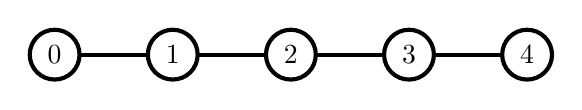
\begin{tikzpicture}
%\draw[help lines] (0,0) grid (6,1);
\SetVertexNormal[
Shape 		= circle,
LineWidth 	= 1.5pt]
\SetUpEdge[
lw 		= 1.5pt,
color 	= black]

\Vertex[x=0,y=1]{0}
\Vertex[x=1.5,y=1]{1}
\Vertex[x=3,y=1]{2}
\Vertex[x=4.5,y=1]{3}
\Vertex[x=6,y=1]{4}

\Edges(0,1,2,3,4)
\end{tikzpicture}
}

\end{frame}

\begin{frame}
\frametitle{2-fold Undo - Wrong}
\begin{center}
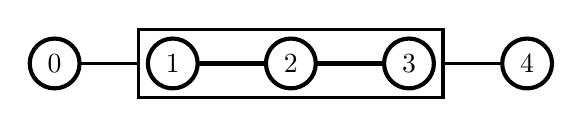
\begin{tikzpicture}
%\draw[help lines] (0,0) grid (6,1);

\SetVertexNormal[
Shape 		= circle,
LineWidth 	= 1.5pt]
\SetUpEdge[
lw 		= 1.5pt,
color 	= black]

\Vertex[x=0,y=1]{0}
\Vertex[x=1.5,y=1]{1}
\Vertex[x=3,y=1]{2}
\Vertex[x=4.5,y=1]{3}
\Vertex[x=6,y=1]{4}

\begin{scope}
\node[fit = (1)(2)(3),draw=black, very thick] (group-inner) {};
\end{scope}

\path[every node/.style={font=\sffamily\small},very thick]
(0.east) edge (group-inner.west)
(group-inner.east) edge (4.west);

\Edges(1,2,3);

\end{tikzpicture}
\end{center}

\end{frame}

\begin{frame}
\frametitle{2-fold Undo - Wrong}
\centering {
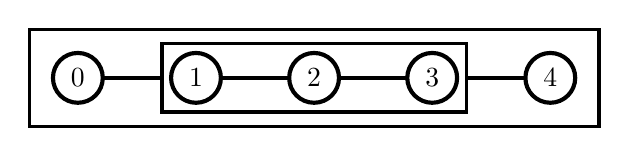
\begin{tikzpicture}
%\draw[help lines] (0,0) grid (6,1);
\SetVertexNormal[
Shape 		= circle,
LineWidth 	= 1.5pt]
\SetUpEdge[
lw 		= 1.5pt,
color 	= black]

\Vertex[x=0,y=1]{0}
\Vertex[x=1.5,y=1]{1}
\Vertex[x=3,y=1]{2}
\Vertex[x=4.5,y=1]{3}
\Vertex[x=6,y=1]{4}


\begin{scope}
\node[fit = (1)(2)(3),draw=black, very thick] (group-inner) {};
\end{scope}
\begin{scope}
\node[fit = (0)(1)(2)(3)(4),draw=black, very thick, inner sep=3mm] (group-outer) {};
\end{scope}

\path[every node/.style={font=\sffamily\small},very thick]
(0.east) edge (group-inner.west)
(group-inner.east) edge (4.west);

\Edges(1,2,3)
\end{tikzpicture}
}
\end{frame}

\begin{frame}
\frametitle{2-fold Undo - Wrong}
\centering {
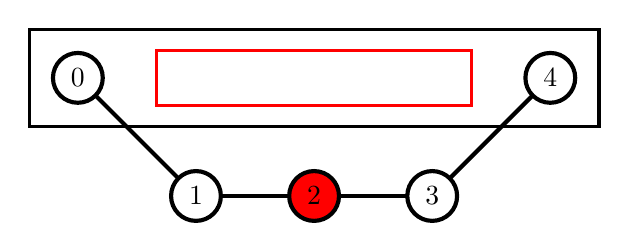
\begin{tikzpicture}
%\draw[help lines] (0,0) grid (6,1);
\SetVertexNormal[
Shape 		= circle,
LineWidth 	= 1.5pt]
\SetUpEdge[
lw 		= 1.5pt,
color 	= black]

\Vertex[x=0,y=1]{0}
\Vertex[x=1.5,y=-0.5]{1}
\Vertex[x=4.5,y=-0.5]{3}
\Vertex[x=6,y=1]{4}

\draw [draw=red,very thick] (1, 0.65) rectangle (5,1.35);
\begin{scope}
\node[fit = (0)(4),draw=black, very thick, inner sep=3mm] (group-outer) {};
\end{scope}

\renewcommand{\VertexLightFillColor}{red}
\Vertex[x=3,y=-0.5]{2}

\Edges(0, 1,2,3,4)
\end{tikzpicture}
}
\end{frame}

\begin{frame}
\frametitle{2-fold Undo - Wrong}
\centering {
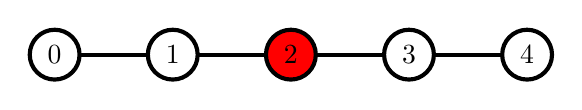
\begin{tikzpicture}
%\draw[help lines] (0,0) grid (6,1);
\SetVertexNormal[
Shape 		= circle,
LineWidth 	= 1.5pt]
\SetUpEdge[
lw 		= 1.5pt,
color 	= black]

\Vertex[x=0,y=1]{0}
\Vertex[x=1.5,y=1]{1}
\Vertex[x=4.5,y=1]{3}
\Vertex[x=6,y=1]{4}

\renewcommand{\VertexLightFillColor}{red}
\Vertex[x=3,y=1]{2}

\Edges(0,1,2,3,4)
\end{tikzpicture}
}
\end{frame}

\begin{frame}
\frametitle{2-fold Undo - Correct}
\centering {
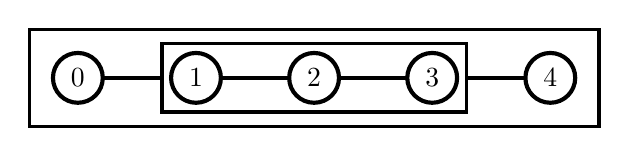
\begin{tikzpicture}
%\draw[help lines] (0,0) grid (6,1);
\SetVertexNormal[
Shape 		= circle,
LineWidth 	= 1.5pt]
\SetUpEdge[
lw 		= 1.5pt,
color 	= black]

\Vertex[x=0,y=1]{0}
\Vertex[x=1.5,y=1]{1}
\Vertex[x=3,y=1]{2}
\Vertex[x=4.5,y=1]{3}
\Vertex[x=6,y=1]{4}


\begin{scope}
\node[fit = (1)(2)(3),draw=black, very thick] (group-inner) {};
\end{scope}
\begin{scope}
\node[fit = (0)(1)(2)(3)(4),draw=black, very thick, inner sep=3mm] (group-outer) {};
\end{scope}

\path[every node/.style={font=\sffamily\small},very thick]
(0.east) edge (group-inner.west)
(group-inner.east) edge (4.west);

\Edges(1,2,3)
\end{tikzpicture}
}
\end{frame}

\begin{frame}
\frametitle{2-fold Undo - Correct}
\centering {
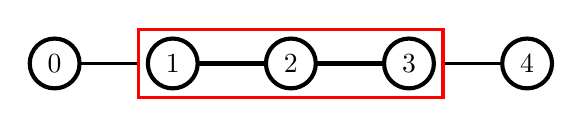
\begin{tikzpicture}
%\draw[help lines] (0,0) grid (6,1);
\SetVertexNormal[
Shape 		= circle,
LineWidth 	= 1.5pt]
\SetUpEdge[
lw 		= 1.5pt,
color 	= black]

\Vertex[x=0,y=1]{0}
\Vertex[x=1.5,y=1]{1}
\Vertex[x=3,y=1]{2}
\Vertex[x=4.5,y=1]{3}
\Vertex[x=6,y=1]{4}

\begin{scope}
\node[fit = (1)(2)(3),draw=red, very thick] (group-inner) {};
\end{scope}

\path[every node/.style={font=\sffamily\small},very thick]
(0.east) edge (group-inner.west)
(group-inner.east) edge (4.west);

\Edges(1,2,3)
\end{tikzpicture}
}
\end{frame}

\begin{frame}
\frametitle{2-fold Undo - Correct}
\centering {
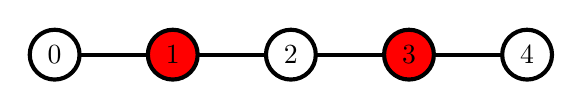
\begin{tikzpicture}
%\draw[help lines] (0,0) grid (6,1);
\SetVertexNormal[
Shape 		= circle,
LineWidth 	= 1.5pt]
\SetUpEdge[
lw 		= 1.5pt,
color 	= black]

\Vertex[x=0,y=1]{0}
\Vertex[x=3,y=1]{2}
\Vertex[x=6,y=1]{4}

\renewcommand{\VertexLightFillColor}{red}
\Vertex[x=1.5,y=1]{1}
\Vertex[x=4.5,y=1]{3}

\Edges(0,1,2,3,4)
\end{tikzpicture}
}
\end{frame}

\begin{frame}
\frametitle{Operation Stack}

Undo order matters!
$\rightarrow$ Stack of operations

\vspace{5mm}

\begin{columns}
\column{0.4\textwidth}
\begin{tabular}{|l|l|}\hline
group 7 & 5 \\ \hline
group  1 & 4 \\ \hline
take 2 & 3 \\ \hline
group 3 & 2 \\ \hline
take 5 & 1 \\ \hline
invalidate 0 & 0\\ \hline
\end{tabular}
\column{0.4\textwidth}
$\Rightarrow 5, 4, 3, 2, 1, 0$
\end{columns}

\vspace{5mm}

Reductions push their operations onto the stack

\end{frame}

\begin{frame}
\frametitle{Configs}
\begin{itemize}[label={$\bullet$}]
\item 8 different reductions\\
$\rightarrow$ Many possible combinations to benchmark
\item Enable/Disable
\item Script can batch execute them
\item Order of application
\item Hierarchy \\
$\rightarrow$ Apply a group of reductions before another
$\rightarrow$ Crown reduction
\end{itemize}
\end{frame}

\begin{frame}
\frametitle{Hierarchy}
\centering{
\begin{forest}
[Data Reduction, tier=zero
[Light, tier=one
[Simple, tier=two, calign=child,calign child=2
[deg0, tier=simple]
[deg1, tier=simple]
[deg2, tier=simple]
[deg $>$ k, tier=simple]
]
[Crown, tier=two
]
]
[Heavy, tier=one
[Dominate, tier=two][Unconfined, tier=two]
]
]
\end{forest}
}

\end{frame}


	\begin{frame}
		\frametitle{Mirror branching}
		
		\vspace*{1cm}
		Mirror branching is a strategy to enhance the standard Max Degree Branching that we use in our implementation. \\
		\vspace*{2cm}
		{\small	Original source is the following paper:\\}
		{\small ``A Measure \& Conquer Approach for the
		Analysis of Exact Algorithms'' by Fedor V. Fomin, Fabrizio Grandoni and Dieter Kratsch}
	\end{frame}
	
	\begin{frame}
		\frametitle{Mirror branching}

		\hspace*{0.8cm}
		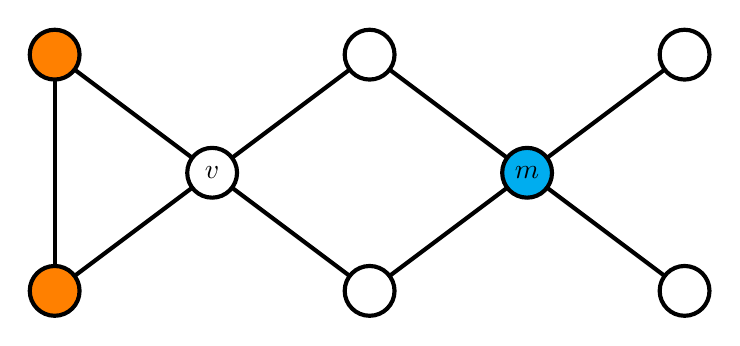
\begin{tikzpicture}
		\SetVertexNormal[
		Shape 		= circle,
		LineWidth 	= 1.5pt]
		\SetUpEdge[
		lw 		= 1.5pt,
		color 	= black]

		

		
		\Vertex[x=5,y=1.5,L=$v$]{2}	
		
		\Vertex[x=7,y=3,L=$ $]{3}
		\Vertex[x=7,y=0,L=$ $]{4}
		
		\Vertex[x=11,y=3,L=$ $]{6}
		\Vertex[x=11,y=0,L=$ $]{7}
		
		\renewcommand{\VertexLightFillColor}{orange}
		
		\Vertex[x=3,y=3,L=$ $ ]{0}
		\Vertex[x=3,y=0,L=$ $]{1}
		
		\renewcommand{\VertexLightFillColor}{cyan}
		\Vertex[x=9,y=1.5,L=$m$]{5}	
		
		\Edges(0,2)
		\Edges(1,2)
		\Edges(0,1)
		
		\Edges(3,2)
		\Edges(4,2)
		
		\Edges(3,5)
		\Edges(4,5)
		
		\Edges(6,5)
		\Edges(7,5)

		
		\end{tikzpicture}


	%	\renewcommand{\VertexLightFillColor}{cyan}

		\vspace*{5mm}
		\hspace*{2.2cm}{\Large 		$ m $ is called \textit{mirror} of $ v $ if:}
		\begin{align*}
		&\text{\large	$\bullet$  $ m \in N^2(v) $}\\
		&\text{\large   $\bullet$  $ N(v) \setminus N(m) $ induces a clique}
		\end{align*}

	
	\end{frame}

	\begin{frame}
	\frametitle{Mirror branching}
	
	\hspace*{0.8cm}
	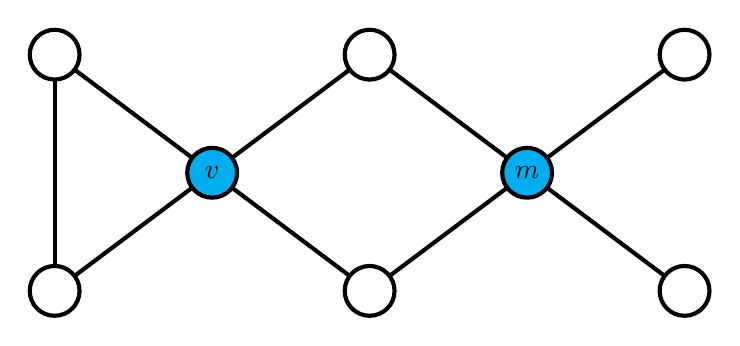
\begin{tikzpicture}
	\SetVertexNormal[
	Shape 		= circle,
	LineWidth 	= 1.5pt]
	\SetUpEdge[
	lw 		= 1.5pt,
	color 	= black]
	
	
	\Vertex[x=3,y=3,L=$ $ ]{0}
	\Vertex[x=3,y=0,L=$ $]{1}
	
	\Vertex[x=7,y=3,L=$ $]{3}
	\Vertex[x=7,y=0,L=$ $]{4}
	
	
	\Vertex[x=11,y=3,L=$ $]{6}
	\Vertex[x=11,y=0,L=$ $]{7}
	
	\renewcommand{\VertexLightFillColor}{cyan}
	\Vertex[x=9,y=1.5,L=$m$]{5}	
	\Vertex[x=5,y=1.5,L=$v$]{2}	

	
	\Edges(0,2)
	\Edges(1,2)
	\Edges(0,1)
	
	\Edges(3,2)
	\Edges(4,2)
	
	\Edges(3,5)
	\Edges(4,5)
	
	\Edges(6,5)
	\Edges(7,5)
	
	
	\end{tikzpicture}
	
	
	\renewcommand{\VertexLightFillColor}{cyan}
	
	\vspace*{5mm}
	\hspace*{2.2cm}{\Large Refined branching rule:}
	\begin{align*}
	&\text{\large	$\bullet$  Either we take $ v $ with all its mirrors into the MVC}\\
	\end{align*}
	
	
	\end{frame}

	\begin{frame}
	\frametitle{Mirror branching}
	
	\hspace*{0.8cm}
	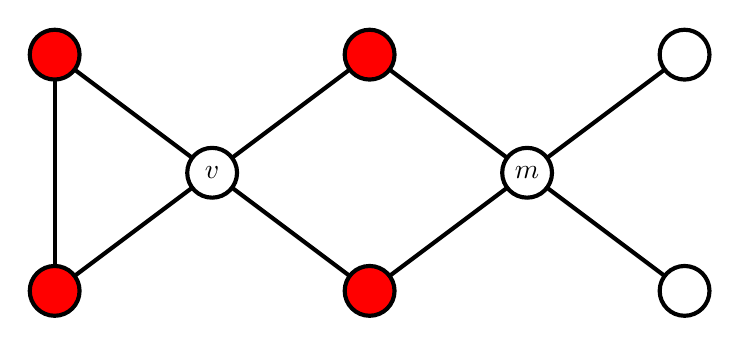
\begin{tikzpicture}
	\SetVertexNormal[
	Shape 		= circle,
	LineWidth 	= 1.5pt]
	\SetUpEdge[
	lw 		= 1.5pt,
	color 	= black]
	
	
	\Vertex[x=5,y=1.5,L=$v$]{2}	
	

	
	\Vertex[x=9,y=1.5,L=$m$]{5}	
	
	\Vertex[x=11,y=3,L=$ $]{6}
	\Vertex[x=11,y=0,L=$ $]{7}
	
	\renewcommand{\VertexLightFillColor}{red}
	\Vertex[x=3,y=3,L=$ $ ]{0}
	\Vertex[x=3,y=0,L=$ $]{1}
	
	\Vertex[x=7,y=3,L=$ $]{3}
	\Vertex[x=7,y=0,L=$ $]{4}
	
	\Edges(0,2)
	\Edges(1,2)
	\Edges(0,1)
	
	\Edges(3,2)
	\Edges(4,2)
	
	\Edges(3,5)
	\Edges(4,5)
	
	\Edges(6,5)
	\Edges(7,5)
	
	
	\end{tikzpicture}
	
	
	%	\renewcommand{\VertexLightFillColor}{cyan}
	
	\vspace*{5mm}
	\hspace*{2.2cm}{\Large Refined branching rule:}
	\begin{align*}
	&\text{\large	$\bullet$  Either we take $ v $ with all its mirrors into the MVC}\\
	&\text{\large   $\bullet$  Or we take $ N(v)$ into the MVC}
	\end{align*}
	\pause
	\vspace*{-5mm}
	\begin{align*}
		{\Large \Rightarrow \text{Always scan for mirrors before branching on a vertex!}}
	\end{align*}
	
	\end{frame}
	
	\begin{frame}
			\frametitle{Mirror branching enhancement}
			
			Previously, we built a branching tree from $ v $ with max size of
			\begin{align*}
				T(n-1) + T(n - |N[v]|)
			\end{align*}
			\pause
			Obviously the search tree is unbalanced.\\
			With mirrors, we attend this issue:\\
			\begin{align*}
				T(n- |\mathcal{M}[v]|) + T(n - |N[v]|)
			\end{align*}
	\end{frame}

	\begin{frame}
	\frametitle{Mirror branching correctness}
	
	\hfil
	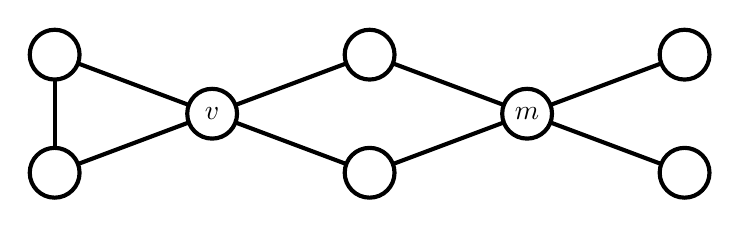
\begin{tikzpicture}
	\SetVertexNormal[
	Shape 		= circle,
	LineWidth 	= 1.5pt]
	\SetUpEdge[
	lw 		= 1.5pt,
	color 	= black]
	
	\Vertex[x=3,y=1.5,L=$ $ ]{0}
	\Vertex[x=3,y=0,L=$ $]{1}
	
	\Vertex[x=5,y=0.75,L=$v$]{2}	
	
	\Vertex[x=9,y=0.75,L=$m$]{5}	
	
	\Vertex[x=11,y=1.5,L=$ $]{6}
	\Vertex[x=11,y=0,L=$ $]{7}
	
	\Vertex[x=7,y=1.5,L=$ $]{3}
	\Vertex[x=7,y=0,L=$ $]{4}
	
	\Edges(0,2)
	\Edges(1,2)
	\Edges(0,1)
	
	\Edges(3,2)
	\Edges(4,2)
	
	\Edges(3,5)
	\Edges(4,5)
	
	\Edges(6,5)
	\Edges(7,5)
	
	
	\end{tikzpicture}
	
	\begin{center}
	Assume we branch on $ v $ and $ v $ has a mirror $ m $.\\
	\pause
	\vspace*{4mm}

	\begin{itemize}
		
		\item[$\rightarrow$]
		\begin{minipage}[t]{25em}
			Then we do not want to include $ N(v) \cap N(m) $ in the MVC.\\
		\end{minipage}\\
		\pause

		\item[$\Rightarrow$]
		\begin{minipage}[t]{25em}
			Because if we did, we might as well just discard $ v $ and cover the clique with its remaining neighbours!
		\end{minipage}
	
	\end{itemize}
	\pause
	\vspace*{5mm}
	\begin{minipage}[t]{20em}
		
		\begin{center}
			Thus, we have to include $ m $ in the MVC \\in order to cover its edges to $ N(v) \cap N(m) $.
		\end{center}

	\end{minipage}

	\end{center}
	
	\end{frame}

	\begin{frame}
		\frametitle{Mirror branching runtime and further heuristics}

			Our implementation finds mirrors of $ v $ in $ O(\delta(v)^3) \leq O(k^3)$, \\
			however it makes use of dynamic programming \\
			to remember already encountered edges.\\
			\pause
			\vspace*{10mm}
			Further branching improvement:\\
			From the max degree vertices, we select the vertex $ v $ that minimizes $ E(N(v)) $.\\
			\pause
			\begin{align*}
				&\rightarrow \text{increases the chance to find mirrors} \qquad\\
				&\rightarrow \text{reduces mirror searching time} \qquad
			\end{align*}

	\end{frame}
	
	\begin{frame}
		\frametitle{Crown Reduction}
		
		Finding crowns is done by computing a maximal matching\\
		$\rightarrow$ non matched vertices form an IS\\
		Build a bipartite graph with V($IS \cup N(IS)$, E) \\
		\pause
		\vspace{5mm}
		
		{\large Observation:}\\
		size of IS depends on the maximal matching\\
		$\rightarrow$ minimum maximal matching is edge dominating set \\ 
		\pause
		$\rightarrow$ our approach: randomize the matching! \\
		
	\end{frame}
		
	\begin{frame}
		\frametitle{Crown Reduction}
		Runtime: \\
		\quad $\mathcal{O} (m \cdot \sqrt{n})$\\
		\vspace{3mm}
		{\large Note: }\\
		\quad n $\rightarrow |IS| + |N(IS)|$ \\
		\quad m $\rightarrow E(IS \cup N(IS))$ \\
		
		\large $\rightarrow$ no guarantee on runtime
	\end{frame}

	\begin{frame}
		\frametitle{0,1}
		\begin{figure}
			\begin{tikzpicture}
			\begin{axis}[
			width=0.8\textwidth,
			height=0.6\textwidth,
			grid,
			xlabel={$n$},
			ylabel={$k$},
			colorbar,
			colorbar style={
				ylabel=time in seconds,
				ylabel style={
					yshift=-7em
				}
			}]
			
			% \thisrowno needs to be used because it does not find the time key for some reason
			\addplot[only marks, color=black, mark=*, scatter] table[x={n}, y={Found VC}, scatter src=\thisrowno{1}, col sep=comma]{../CSVs/FINAL_0_and_1_random_out.csv};
			
			\addplot[only marks, color=black, mark=+, scatter] table[x={n}, y={Found VC}, scatter src=\thisrowno{1}, col sep=comma]{../CSVs/FINAL_0_and_1_dimacs_out.csv};
			
			\addplot[only marks, color=black, mark=triangle*, scatter] table[x={n}, y={Found VC}, scatter src=\thisrowno{1}, col sep=comma]{../CSVs/FINAL_0_and_1_snap_out.csv};
			\end{axis}
			\end{tikzpicture}
		\end{figure}
	\end{frame}

	\begin{frame}
	\frametitle{0,1,2,k,dominate}
	\begin{figure}
		\begin{tikzpicture}
		\begin{axis}[
		width=0.8\textwidth,
		height=0.6\textwidth,
		grid,
		xlabel={$n$},
		ylabel={$k$},
		colorbar,
		colorbar style={
			ylabel=time in seconds,
			ylabel style={
				yshift=-7em
			}
		}]
		
		% \thisrowno needs to be used because it does not find the time key for some reason
		\addplot[only marks, color=black, mark=*, scatter] table[x={n}, y={Found VC}, scatter src=\thisrowno{1}, col sep=comma]{../CSVs/FINALPLUS_0_and_1_and_2_k_dominate_random_out.csv};
		
		\addplot[only marks, color=black, mark=+, scatter] table[x={n}, y={Found VC}, scatter src=\thisrowno{1}, col sep=comma]{../CSVs/FINALPLUS_0_and_1_and_2_k_dominate_dimacs_out.csv};
		
		\addplot[only marks, color=black, mark=triangle*, scatter] table[x={n}, y={Found VC}, scatter src=\thisrowno{1}, col sep=comma]{../CSVs/FINALPLUS_0_and_1_and_2_k_dominate_snap_out.csv};
		\end{axis}
		\end{tikzpicture}
	\end{figure}
\end{frame}

	\begin{frame}
	\frametitle{0,1,2,k,unconfined}
	\begin{figure}
		\begin{tikzpicture}
		\begin{axis}[
		width=0.8\textwidth,
		height=0.6\textwidth,
		grid,
		xlabel={$n$},
		ylabel={$k$},
		colorbar,
		colorbar style={
			ylabel=time in seconds,
			ylabel style={
				yshift=-7em
			}
		}]
		
		% \thisrowno needs to be used because it does not find the time key for some reason
		\addplot[only marks, color=black, mark=*, scatter] table[x={n}, y={Found VC}, scatter src=\thisrowno{1}, col sep=comma]{../CSVs/FINALPLUS_0_and_1_and_2_k_unconfined_random_out.csv};
		
		\addplot[only marks, color=black, mark=+, scatter] table[x={n}, y={Found VC}, scatter src=\thisrowno{1}, col sep=comma]{../CSVs/FINALPLUS_0_and_1_and_2_k_unconfined_dimacs_out.csv};
		
		\addplot[only marks, color=black, mark=triangle*, scatter] table[x={n}, y={Found VC}, scatter src=\thisrowno{1}, col sep=comma]{../CSVs/FINALPLUS_0_and_1_and_2_k_unconfined_snap_out.csv};
		\end{axis}
		\end{tikzpicture}
	\end{figure}
\end{frame}

\begin{frame}
\frametitle{0,1,2,k,dominate, unconfined}
\begin{figure}
	\begin{tikzpicture}
	\begin{axis}[
	width=0.8\textwidth,
	height=0.6\textwidth,
	grid,
	xlabel={$n$},
	ylabel={$k$},
	colorbar,
	colorbar style={
		ylabel=time in seconds,
		ylabel style={
			yshift=-7em
		}
	}]
	
	% \thisrowno needs to be used because it does not find the time key for some reason
	\addplot[only marks, color=black, mark=*, scatter] table[x={n}, y={Found VC}, scatter src=\thisrowno{1}, col sep=comma]{../CSVs/FINAL_all_except_crown_random_out.csv};
	
	\addplot[only marks, color=black, mark=+, scatter] table[x={n}, y={Found VC}, scatter src=\thisrowno{1}, col sep=comma]{../CSVs/FINAL_all_except_crown_dimacs_out.csv};
	
	\addplot[only marks, color=black, mark=triangle*, scatter] table[x={n}, y={Found VC}, scatter src=\thisrowno{1}, col sep=comma]{../CSVs/FINAL_all_except_crown_snap_out.csv};
	\end{axis}
	\end{tikzpicture}
\end{figure}
\end{frame}

\begin{frame}
\frametitle{0,1,2,k,crown}
\begin{figure}
	\begin{tikzpicture}
	\begin{axis}[
	width=0.8\textwidth,
	height=0.6\textwidth,
	grid,
	xlabel={$n$},
	ylabel={$k$},
	colorbar,
	colorbar style={
		ylabel=time in seconds,
		ylabel style={
			yshift=-7em
		}
	}]
	
	% \thisrowno needs to be used because it does not find the time key for some reason
	\addplot[only marks, color=black, mark=*, scatter] table[x={n}, y={Found VC}, scatter src=\thisrowno{1}, col sep=comma]{../CSVs/FINAL_all_except_unconfined_and_dominate_random_out.csv};
	
	\addplot[only marks, color=black, mark=+, scatter] table[x={n}, y={Found VC}, scatter src=\thisrowno{1}, col sep=comma]{../CSVs/FINAL_all_except_unconfined_and_dominate_dimacs_out.csv};
	
	\addplot[only marks, color=black, mark=triangle*, scatter] table[x={n}, y={Found VC}, scatter src=\thisrowno{1}, col sep=comma]{../CSVs/FINAL_all_except_unconfined_and_dominate_snap_out.csv};
	\end{axis}
	\end{tikzpicture}
\end{figure}
\end{frame}
\begin{frame}
\frametitle{All Reductions}
\begin{figure}
	\begin{tikzpicture}
	\begin{axis}[
	width=0.8\textwidth,
	height=0.6\textwidth,
	grid,
	xlabel={$n$},
	ylabel={$k$},
	colorbar,
	colorbar style={
		ylabel=time in seconds,
		ylabel style={
			yshift=-7em
		}
	}]
	
	% \thisrowno needs to be used because it does not find the time key for some reason
	\addplot[only marks, color=black, mark=*, scatter] table[x={n}, y={Found VC}, scatter src=\thisrowno{1}, col sep=comma]{../CSVs/FINAL_config_example_random_out.csv};
	
	\addplot[only marks, color=black, mark=+, scatter] table[x={n}, y={Found VC}, scatter src=\thisrowno{1}, col sep=comma]{../CSVs/FINAL_config_example_dimacs_out.csv};
	
	\addplot[only marks, color=black, mark=triangle*, scatter] table[x={n}, y={Found VC}, scatter src=\thisrowno{1}, col sep=comma]{../CSVs/FINAL_config_example_snap_out.csv};
	\end{axis}
	\end{tikzpicture}
\end{figure}
\end{frame}

\begin{frame}
	\frametitle{Unconfined and Dominate Comparison}
	
	\begin{tikzpicture}[scale=1]
	\begin{loglogaxis}[
	width=0.9\textwidth,
	height=0.55\textwidth,
	xlabel={Unconfined},
	ylabel={Dominate},
	xmin=1,
	ymin=1]
	
	\addplot[only marks,color=orange,mark=triangle*] table [y={Recursive Steps}, x={rec_uncon},col sep=semicolon] {../CSVs/uncon_domi_snap.csv};
	
	\addplot+[mark=none,black,domain=1:10000] {x};
	
	\addplot[only marks,color=orange,mark=+] table [y={Recursive Steps}, x={rec_uncon},col sep=semicolon] {../CSVs/uncon_domi_dimacs.csv};
	% helper lines 
	%\addplot[color=black] {x};
	%\addplot[dashed,color=black!75,domain=\minValue:\maxValue,samples=4] {5*x};
	%\addplot[dashed,color=black!75,domain=\minValue:\maxValue,samples=4] {0.2*x};
	%\addplot[dotted,color=black,domain=\minValue:\maxValue,samples=4] {25*x};
	%\addplot[dotted,color=black,domain=\minValue:\maxValue,samples=4] {0.04*x};
	\end{loglogaxis}
	\end{tikzpicture}
\begin{center}
		*Only instances solved by both variants are listed*
\end{center}
\end{frame}

\begin{frame}
\frametitle{0 and 1 to All Reductions comparison}

\begin{tikzpicture}[scale=1]
\begin{loglogaxis}[
width=0.9\textwidth,
height=0.55\textwidth,
xlabel={All Reductions},
ylabel={0 and 1 Reduction},
xmin=1,
ymin=1]

\addplot[only marks,color=orange,mark=triangle*] table [y={Recursive Steps}, x={rec_all},col sep=semicolon] {../CSVs/1_to_all_snap.csv};

\addplot+[mark=none,black,domain=1:100000] {x};

\addplot[only marks,color=orange,mark=+] table [y={Recursive Steps}, x={rec_all},col sep=semicolon] {../CSVs/1_to_all_dimacs.csv};
% helper lines 
%\addplot[color=black] {x};
%\addplot[dashed,color=black!75,domain=\minValue:\maxValue,samples=4] {5*x};
%\addplot[dashed,color=black!75,domain=\minValue:\maxValue,samples=4] {0.2*x};
%\addplot[dotted,color=black,domain=\minValue:\maxValue,samples=4] {25*x};
%\addplot[dotted,color=black,domain=\minValue:\maxValue,samples=4] {0.04*x};
\end{loglogaxis}
\end{tikzpicture}
\begin{center}
	*Only instances solved by both variants are listed*
\end{center}
\end{frame}

\begin{frame}
\frametitle{Components}
\begin{itemize}
	\item $1$. Use DFS to find components
	\item $2$. Create subgraphs for each component
	\item $3$. Sort them to process easy ones first
	\item $4$. Solve on each subgraph
	\item $5$. Combine the found solutions
\end{itemize}
\vspace{5mm}
Faster because we break earlier and reduce k early.

\end{frame}


\begin{frame}
%TODO some conclusions and an outlook to what we will be doing
\frametitle{Outlook on Future Improvements}

\begin{itemize}
	\item[-] Performance Improvements for Reductions
	\item[-] LP reduction via Flow
	\item[-] Degree 3 reduction
	\item[-] Refactor Solver
	\item[-] Priority Queue for Vertex Selection
\end{itemize}




\end{frame}
\begin{frame}
\frametitle{Thanks for your attention}
\centering	\Huge Questions?
\end{frame}




\end{document}